% Created 2024-10-16 śro 21:35
% Intended LaTeX compiler: pdflatex
\documentclass[../main.tex]{subfiles}

% \usepackage[a4paper, margin=3cm]{geometry}
% \usepackage{amssymb} // not working

\usepackage[T1]{fontenc}
\usepackage[utf8]{inputenc}
\usepackage{graphicx}
\usepackage{longtable}
\usepackage{wrapfig}
\usepackage{rotating}
\usepackage[normalem]{ulem}
\usepackage{amsmath}
\usepackage{capt-of}
\usepackage{hyperref}
\usepackage{siunitx}
\usepackage{float}
\usepackage[polish]{babel}

\graphicspath{{../}}
\author{Wojciech Paderewski}
\date{\today}
\title{Lampy nixie}
\hypersetup{
 pdfauthor={Wojciech Paderewski},
 pdftitle={Lampy nixie},
 pdfkeywords={},
 pdfsubject={},
 pdflang={Polish}}

\begin{document}

Lampy nixie są to szklane lampy wyświetlające cyfry, litery lub inne symbole.
Składa się z katod w kształcie cyfr, liter lub innych symboli oraz anode w kształcie siatki, wszystkie
te elementy zamknięte są w szklanej bańce wypełnionej gazem szlachetnym.
Wyświetlenie danej cyfry odbywa się poprzez wysterowanie odpowiedniej katody.

Nixie były używane w latach 50-70 XX wieku w różnych urządzeniach pomiarowych, licznikach, zegarach, itp. 
Obecnie nie są używane ze względu na konieczność zasilania wysokim napięciem, skomplikowanie układu sterującego i duży koszt produkcji.
Mają one natomiast ponadczasowe walory estetyczne, co jest powodem ich popularności pośród elektroników hobbystów.

\subsection{Zasada działania}
Zjawisko zachodzące w lampach zwane jest jako wyładowanie gazowe.\cite{st:nixie}
Naładowane elektrycznie cząstki (elektrony), poprzez wysokie napięcie osiągają dużą energię kinetyczną.
W momencie zderzenia z atomami gazu, elektrony w atomie gazu są wzbudzane do wyższych stanów energetycznych, a następnie wracają do stanu podstawowego emitując foton światła.

Barwa światła zależy od gazu:
\begin{itemize}
  \item jony neonu - czerwono-pomarańczowe,
  \item wodór - niebieskawo-fioletowy,
  \item azot - fiolet,
  \item krypton - biało-niebiesko.
\end{itemize}

Najczęściej stosowana jest mieszanka neonu i argonu pod małym ciśnieniem. Dodawana jest również rtęć, 
która ma za zadanie zwiększyć trwałość lampy, 
minimalizując tak zwane zatrucie katodowe. Efekt ten powoduje nie pełne pokrycie katody warstwą gazową, c
o powoduje zanikanie wyświetlania cyfr,
a czasami skutkuje zanikiem wyświetlania całkowicie.

\begin{figure}[H]
  \centering
  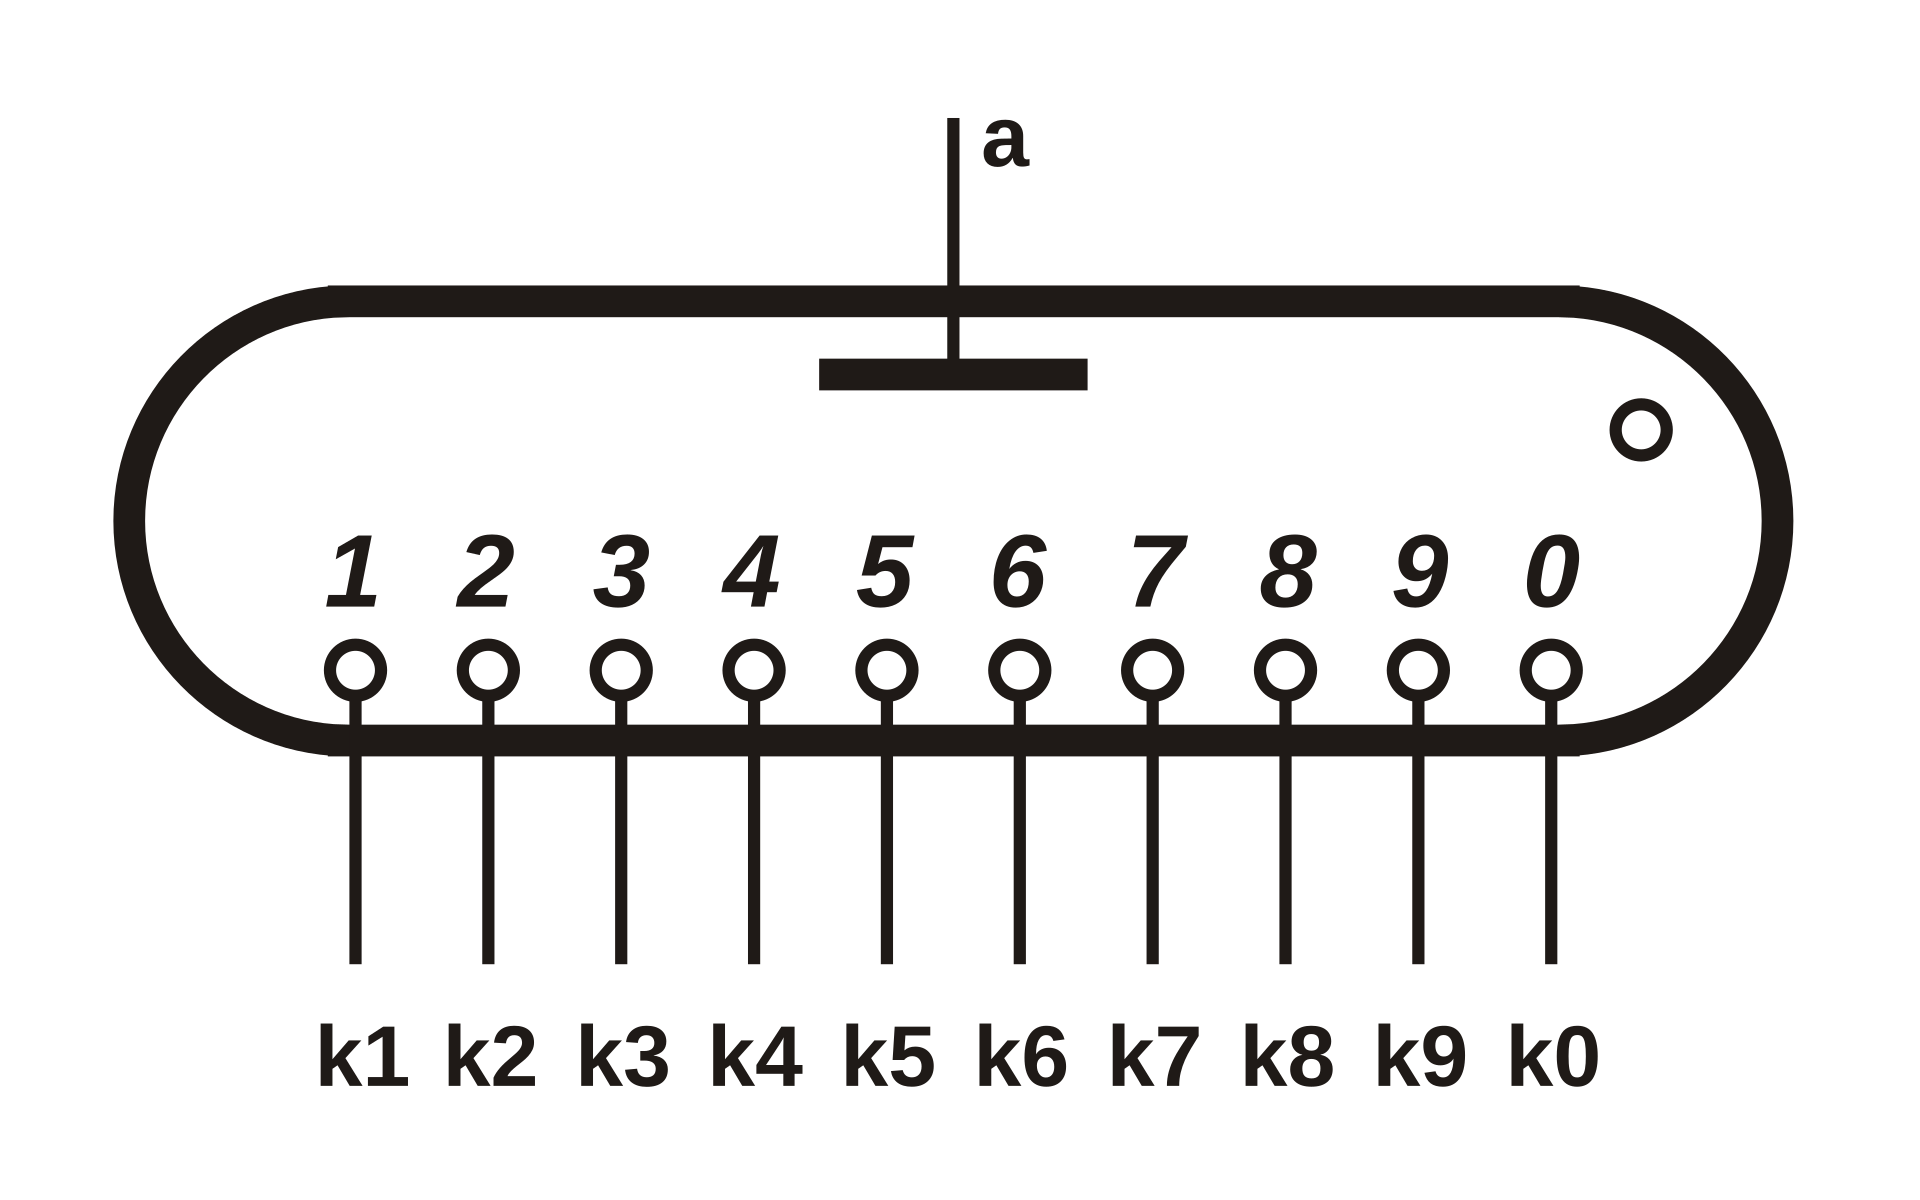
\includegraphics[width=0.5\textwidth]{Nixie_schematic.png}
  \caption{Schemat elektryczny lampy nixie ze wspólną anodą\cite{st:nixie-jpg}}
\end{figure}

Najczęściej spotykaną konfiguracją podłączenia lampy jest wspólna anoda, gdzie katody są sterowane sygnałem, a anoda jest podłączona
do zasilanie przez rezystor ograniczający prąd. W przypadku lampy nixie, napięcie zasilanie wynosi od \SI{150}{\volt} do \SI{200}{\volt}.

\subsection{Problemy związane z wykorzystaniem lamp nixie}

Lampy są podatne na wiele problemów, które mogą wystąpić podczas użytkowania, takie jak:
\begin{itemize}
  \item \textbf{Zatrucie katodowe} - zanikanie wyświetlania cyfr, spowodowane nie pełnym pokryciem katody warstwą gazową.
  \item \textbf{Zjawisko kropkowania} - zjawisko polegające na wyświetlaniu kropek w miejscach gdzie nie powinny się one znajdować.
  \item \textbf{Zjawisko spalania} - zjawisko polegające na spalaniu się katod, spowodowane zbyt dużym prądem płynącym przez katodę.
  \item \textbf{Zjawisko cienia} - zjawisko polegające na wyświetlaniu niebieskiej poświaty, spowodowane zbyt dużym napięciem na anodzie.
  \item \textbf{Zjawisko zaniku} - zjawisko polegające na zanikaniu wyświetlania cyfr, spowodowane zbyt małym napięciem na anodzie.
\end{itemize}

Największym problemem jest zatrucie katodowe w szczególności w kontekście lamp używanych w zegarach nixie. 
Tylko parzyste wyświetlacze działają w optymalny sposób, ponieważ używają wszystkich cyfr, 
a więc wszystkie cyfry zużywają się równomiernie.
Problem pojawia się w przypadku nieparzystych katod, gdzie niektóre cyfry są używane znacznie rzadziej niż inne.

Na przykład, lampa po skrajnej lewej stronie wykorzystuje cyfry 0, 1, 2 do wyświetlania części dziesiętnej godziny.
Trzecia lampa (pozycja dziesiątek minut) używa cyfr 0, 1, 2, 3, 4, 5. Gdy konkretna cyfra nie jest używana przez długi czas
 (np. cyfra 8 na najbardziej po lewej stronie lampy),
cyfra ta jest pokryta osadem metalu uwolnionym z innych aktywowanych cyfr.
 Te konkretne cyfry ostatecznie będą miały defekty w świeceniu, jeżeli nie zostaną użyte przez długi czas.

\subsection{Rozwiązania problemów związanych z lampami nixie}
Rozwiązaniem problemu zatrucia katodowego jest sterowanie lampami w taki sposób, aby wszystkie cyfry były używane.
Można to osiągnąć na przykład poprzez animacje, gdy zmienia się cyfra minut.
Można również w godzinach nocnych przez jakiś czas wyświetlać cyklicznie wszystkie cyfry, aby zapobiec zatruciu katodowemu.

W celu zwiększenia trwałości lamp można również tak sterować lampami, aby zmniejszyć prąd pracy lampy. Ogranicza to
 zjawisko spalania katod, natomiast prąd musi być wystarczająco duży aby lampa świeciła jasno.

\newpage

\subsection{Sterowanie lampami}
\label{sec:sterownie_lampi}

Sterowanie lampami nixie jest trudne ze względu na konieczność zastosowania wysokiego napięcia.
Przy szacowaniu potrzebnych pinów i elementów założono użycie 6 lamp nixie, każda lampa ma 10 katod z cyframi od 0 do 9 oraz 
kropkę dziesiętną, co daje 11 sygnałów sterujących na lampę.
Istnieje kilka sposobów sterowania lampami nixie\cite{st:nixie1}:

\begin{itemize}
    \item Sterowanie bezpośrednie - każda lampa ma swoje wejście i jest sterowana osobno za pomocą tranzystora HV połączonego z mikrokontrolerem.
    Wadą jest konieczność posiadania wielu pinów GPIO, co jest nieoptymalne. Sumarycznie wymaga to 66 pinów GPIO oraz 66 tranzystorów HV.
    Można by w tym porzadku zastosować multipleksery co zmniejszyło by ilość wymaganych pinów GPIO do 16, ale zwiększa to skomplikowanie układu.
    \item Multiplexing - wszystkie lampy są podłączone do jednego drivera, który wybiera katode i załącza odpowiednią anodę. 
    Wymaga to mniej pinów GPIO bo tylko 10, ale multipleksacja powoduje szybsze zużycie lamp i pojawia się artefaktów.
    \item Wykorzystanie dedykowanych driverów - istnieją specjalne układy scalone, które są przeznaczone do sterowania lampami nixie, niestety
    one również wymagają wielu pinów GPIO po 4 na każdą lampę, co daje 24 wymagane piny GPIO.
    \item Rejestr przesuwny HV - najbardziej optymalne rozwiązanie, wymaga tylko 3 pinów GPIO. Rejestry HV są ciężko dostępne i dość drogie,
    muszą też posiadać zatrzask. Wymagane jest również by rejestry miały wyjścia typu Open Drain.
    \item Połączenie rejestrów przesuwnych z driverami - połączenie rejestrów przesuwnych HV z dedykowanymi driverami, pozwala na zastosowania
    rejestru przesuwnego dla niskiego napięcia. Ta kombinacja również wymaga 3 pinów GPIO, przy rejestrze 32 bitowym i 6 driverach. Powoduje jednak to
    większe skomplikowanie układu oraz układ taki zajmuje więcej miejsca.
\end{itemize}

%tabela opłacalności czyli : nazwa, ilość pinów, cena, trudność w implementacji, zajętość miejsca
\begin{table}[H]
  \centering
  \begin{tabular}{|c|c|c|c|c|}
    \hline
    Nazwa & Ilość pinów & Cena & Trudność implementacji & Objętość\\
    \hline
    Sterowanie bezpośrednie & 66 & niska-średnia & niska-średnia & duża \\
    \hline
    Multiplexing & 10 &niska & wysoka & mała \\
    \hline
    Dedykowane drivery & 24 &średnia & niska & średnia \\
    \hline
    Rejestr przesuwny HV & 3 &wysoka & niska & średnia \\
    \hline
    Rejestr przesuwny + drivery & 3 & wysoka & średnia & duża \\
    \hline
  \end{tabular}
  \caption{Tabela opłacalności sposobów sterowania lampami nixie}
\end{table}

\subsection{Sytuacja na rynku}
Obecnie dostępność lamp nixie jest ograniczona, gdyż nie są one już produkowane masowo. Istnieją małe firmy, które zajmują się produkcją, ale są to bardzo
duże lampy w małych ilościach, co powoduje ich wysoką cenę. Dostępne są również lampy używane, ale w tym przypadku również duże lampy są drogie, a małe lampy są trudne do znalezienia.
Problemem jest również nie wiadomy stan lamp, ponieważ są to produkty one używane.

\end{document}
